\documentclass[fr]{../../../../../../eplexam}

\hypertitle{matstruct-GCIV1031}{4}{GCIV}{1031}{2015}{Juin}
{Geoffroy Jacquet\and L\'{e}a Paulus}
{Jean-François Cap et Denis Zastavni}

\part{Série 1}
\section{Citer les 3 différents types de solides + exemple pour chacun}
\begin{solution}
\begin{enumerate}
\item Les solides cristallins (l'acier)
\item Les solides non-cristallins (le verre)
\item Les solides semi-cristallins (polymère thermoplastique)
\end{enumerate}
\end{solution}

\section{Différence entre action directe/ indirecte + exemple}
\begin{solution}
Une action est une cause produisant un jeu de forces dans une une construction. Les directes sont représentées sous forme de forces extérieures, appelées charges (Ex: le vent). Les indirectes font naitre des jeux  de force interne dans la structure (Ex: variation de la température).
\end{solution}

\section{Dessiner le graphe du fluage des métaux à haute températures, pour des contraintes croissantes}
\begin{solution}
\begin{center}
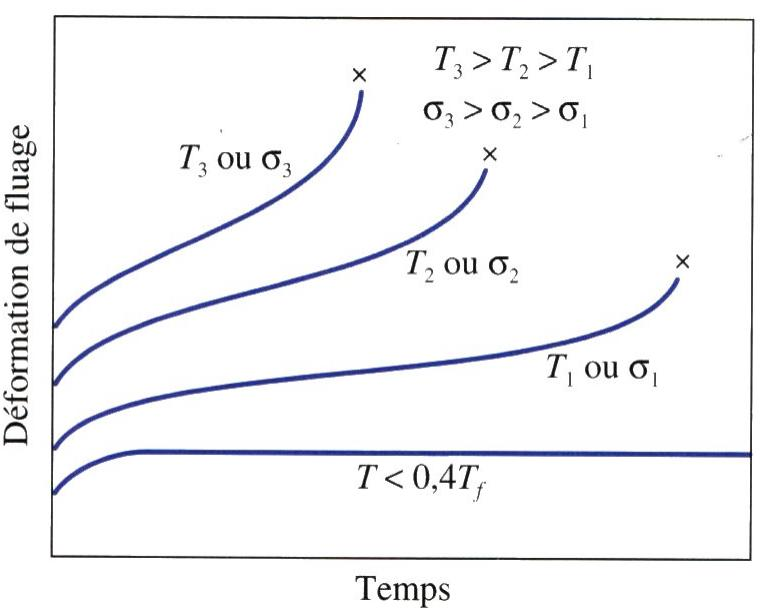
\includegraphics[scale=0.23]{fluage_temp.jpg}
\quad
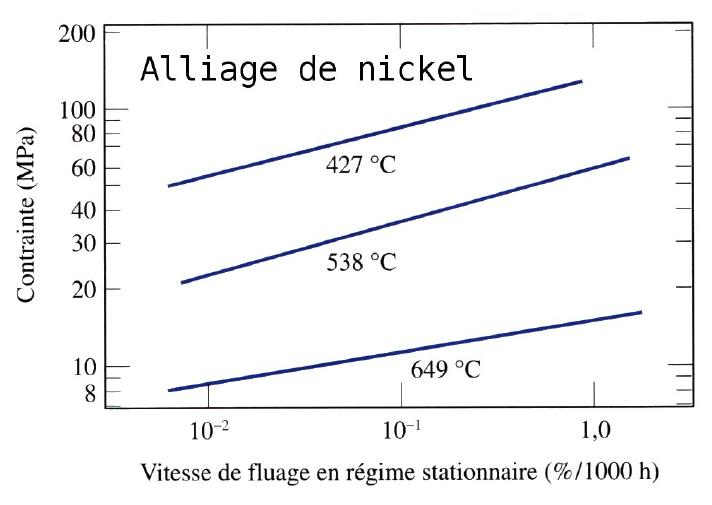
\includegraphics[scale=0.3]{fluage_temp2.jpg}
\end{center}
\end{solution}

\section{Donner les différentes couches du bois + leur rôle}
\begin{solution}
\begin{enumerate}
\item L’écorce: cellules mortes.
\item Le liber: Zone de croissance de l'écorce.
\item Le cambium: zone de croissance de bois du tronc.
\item L'aubier: zone de bois vivante qui véhicule la sève.
\item Le duramen: zone quasi inerte qui sert de structure à l'arbre.
\item La moelle: zone qui a servi à la formation initiale.
\end{enumerate}
\end{solution}

\section{Donner 2 quantifiant de la ductilité d'un métal}
\begin{solution}
\begin{enumerate}
\item Pourcentage de la déformation à la rupture: défini pour une distance entre 2 points de mesure conventionnelle $I_0$ et $I_F$ et cette même distance mesurée après la rupture.
\item Coefficient de striction: défini à partir de la section initiale  $S_0$ de l'éprouvette et la section au point de rupture $S_f$.
\end{enumerate}
\end{solution}

\section{Donner les différents type de façonnage d'une brique}
\begin{solution}
\begin{enumerate}
\item Briques moulées main.
\item Briques pressées.
\item Briques étirées.
\end{enumerate}
\end{solution}

\section{Un polycristallin est-il isotrope/anisotrope, expliquer pourquoi}
\begin{solution}
Bien que chaque grain se comporte de manière anisotrope, l'orientation cristallographique des grains étant complètement aléatoire, l’échantillon se comportera de manière isotrope.
\end{solution}

\section{Citer les défauts ponctuels}
\begin{solution}
\begin{itemize}
\item Les lacunes.
\item Les atomes auto-interstitiels.
\item Les impuretés.
\item Les solutions solides.
\end{itemize}
\end{solution}

\section{Expliquer le recuit de détente}
\begin{solution}
Utilisé pour éliminer les contraintes résiduelles, on chauffe assez longtemps afin que toutes les parties soient à la même température (prédéfinie) et on laisse ensuite refroidir à température ambiante.
\end{solution}

\section{Définir le diagramme de contrainte-déformation du béton en compression}
\begin{solution}
\begin{center}
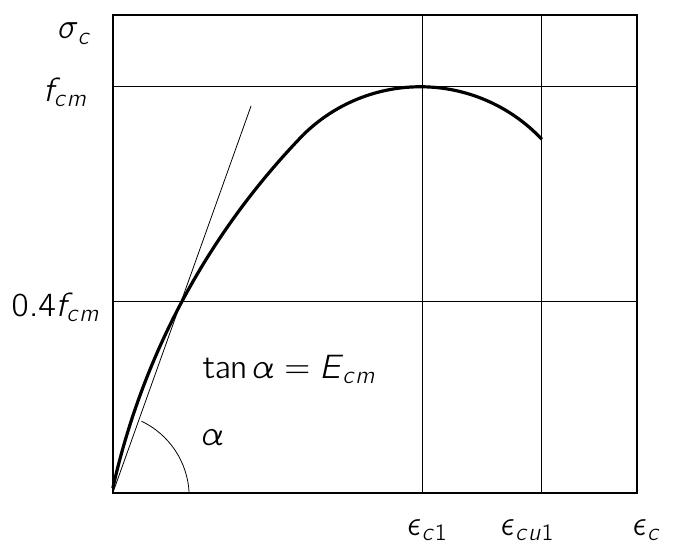
\includegraphics[scale=0.3]{beton_CD.jpg}

\end{center}
\end{solution}

\section{Définir la dureté d'un matériaux}
\begin{solution}
La dureté exprime la résistance d'un matériaux soumis à une déformation plastique localisée (par exemple une petite indentation ou rayure).
\end{solution}

\section{Pourquoi la maçonnerie peut être vue comme un comportement plastique ideal}
\begin{solution}
Si l'on met en compression une maçonnerie (par exemple sous son poids propre), on pourrait lui apporter une résistance en traction : celle pour retirer la charge appliquée. Sauf qu'une fois en traction, la maçonnerie se défait à l'infini : elle est donc parfaitement plastique et rigide (pente de E verticale, puis totalement horizontale). En compression, on a un comportement fort proche si on triche un peu sur les échelles du diagramme contrainte-défo. On applique donc un calcul plastique sur un assemblage fragile.
\end{solution}

\section{Définir la dilatation thermique}
\begin{solution}
A l'échelle atomique, la dilatation thermique correspond à une augmentation de la distance entre les atomes.

\end{solution}

\section{Définir l'anélasticité}
\begin{solution}
Composante de déformation élastique dépendante du temps, la déformation élastique se poursuit donc après l’application de la contrainte et ne s'annule qu'au bout d'un certain temps après la suppression de la charge.
\end{solution}

\section{Quelle est l'unité de mesure de l'essai Charpy et en quoi consiste-t-il}
\begin{solution}
L'unité de mesure est celle de l'énergie c'est-à-dire des Joule. L'essai de Charpy consiste en une éprouvette placée au bas de l'appareil. Après la libération d'un mouton pendule, un couteau monté sur celui-ci vient frapper l'éprouvette et la rompt à l'entaille, qui devient un point de concentration des contraintes lors de ce choc à haute vitesse. Le pendule poursuit sont mouvement et s'élève à une hauteur maximale 
$h'$, inférieure à $h$. L'énergie absorbée, calculée à partie de $h'$ et $h$ équivaut à l'énergie de rupture.
\end{solution}

\section{Définir le concept de fatigue}
\begin{solution}
La fatigue est une forme de défaillance qui se produit dans t des structures subissant des contraintes dynamiques et variables
\end{solution}

\section{Quel effet à l'ajout d'un plastifiant au béton}
\begin{solution}
En maintenant une qualité constante ($\frac{E}{C}$ constant), on peut gagner une classe de consistance.
\end{solution}

\section{Qu'est-ce qui influence principalement la qualité d'un ciment}
\begin{solution}
Le paramètre eau/ciment ($\frac{E}{C}$).
\end{solution}

\section{Citer les 3 familles de bois et donner leurs propriétés}
\begin{solution}
\begin{itemize}
\item Les résineux: plus légers, souvent utilisés pour les structures, droits et longs.
\item Les feuillus à bois durs: plus lourd, utilisés pour le mobiliers et les escaliers, plus durables que les résineux.
\item Les tropicaux: plus durables, utilisé pour les châssis de fenêtre, les revêtements de sol extérieur.
\end{itemize}
\end{solution}

\section{Quel est l'effet du chargement maintenu sur une poutre de béton en compression}
\begin{solution}
une augmentation de la déformation au cours du temps sous une charge constante ainsi qu'une production de micros-fissures se propageant lentement.
\part{Série 2}
\end{solution}

\section{Définir une liaison métallique}
\begin{solution}
La matériaux métalliques peuvent avoir un, deux ou au plus trois électrons de valence. Ces électrons de valences ne sont liés à aucun atome particulier du solide et sont pratiquement libres de circuler à travers le métal tout entier. On peut imaginer qu'ils appartiennent à la totalité du métal, ou qu'ils forment un nuages d'électrons.
\end{solution}

\section{Définir un matériau anisotrope}
\begin{solution}
Substance dont les propriétés sont dépendantes de la direction de la mesure.
\end{solution}

\section{Définir la perlite}
\begin{solution}
La perlite est une microstructure de l'acier eutectoïde constitué de couches alternées des ferrite et de cémentite. 
\end{solution}

\section{De quoi sont composés les blocs silico-calcaire et quelles sont les étapes de leur fabrication}
\begin{solution}
Ils sont composés à partir d'un mélange de sable, de chaux et d'eau. Leurs étapes de fabrications sont les suivantes:
\begin{enumerate}
\item Dosage du mélange sable (90\%) + chaux vive (7\%) et d'eau (3\%).
\item Mélange intensif puis stockage 4h en réacteur.
\item Mélange et correction de l'humidité du mélange.
\item pressage à 15 bars et $200^{\circ}$C.
\item passage en autoclave (6h).
\item emballage et expédition.
\end{enumerate}

\end{solution}

\section{Quels sont les constituants du bois qui entraînent une variation dimensionnelle}
\begin{solution}
L'eau liée provoque le gonflement transversal du bois. Et l'eau libre occupant les vides cellulaires du bois.
\end{solution}

\section{Quels sont les différents liants disponibles pour un mortier}
\begin{solution}
La chaux aérienne, la chaux hydraulique, le plâtre (semi-hydraté), le plâtre anhydraté et le ciment.
\end{solution}

\section{Donner 5 exemples de produits dérivés du bois et leur(s) usage(s) en construction}
\begin{solution}
\begin{enumerate}
\item Panneau massif: façade
\item Panneau de bois lamifié: poutres et châssis.
\item Éléments massifs contre-collé: parois ou planchers.
\item Laminated Strand Lumber: linteaux, pannes et poutres
\item Parallel Strand Lumber: poutres et poteaux.
\end{enumerate}
\end{solution}

\section{Dessiner le diagramme de l'essai de Charpy de l'acier à différentes températures}
\begin{solution}
\end{solution}

\section{Comment mesure-t-o  la dureté d'un matériau}
\begin{solution}
Pour calculer la dureté d'un matériau en fait entrer de force un pénétrateur dont les dimensions sont standardisées dans la surface du matériau, la dureté se déduit de l'entaille ainsi réalisée.
\end{solution}

\section{Définir le modèle de Hooke}
\begin{solution}
Le déplacement $\delta$ est proportionnel à la force $F$ moyennant une constance de raideur $M$.
$$F=M\delta$$
Les déformations de l’élément sont  instantanées et complètement réversibles.
\end{solution}

\section{Donner les différents composés hydrauliques qui sortent d'un four de cimenterie}
\begin{solution}
L'alite, silicate tricalcique (60\%), la bélite, silicate bicalcique (20\%), la célite, mélange d'aluminate (10\%), d'alumino-ferrite tétracalcique (10\%).
\end{solution}

\section{Schématiser le diagramme contrainte déformation du caoutchouc lors d'un traction uni-axiale}
\begin{solution}
\begin{center}
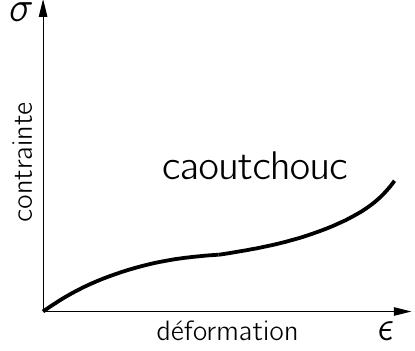
\includegraphics[scale=0.4]{Caoutchouc_CD.jpg}
\end{center}

\end{solution}

\section{Différence entre contrainte réelle et contrainte nominale}
\begin{solution}
La contrainte réelle est la force sur la section transversale du matériaux allongé tandis que la contrainte nominale est la force sur la section nominale du matériau avant qu'il soit allongé.
\end{solution}

\section{Qu'est-ce que le procédé de cémentation}
\begin{solution}
La cémentation est un procédé permettant d'augmenter la dureté en surface et la durée de vie en fatigue des aciers, consiste à traiter une pièce par enrichissement en carbone ou par nitruration en l'exposant à une atmosphère carbonée ou azotée à haute température.
\end{solution}

\section{Qu’est ce qu’une solution solide d’insertion}
\begin{solution}
C'est un défaut ponctuel formé lorsque l'addition d'impureté ne modifie pas la structure cristalline d'une matière hôte.
Dans ce cas les atomes d'impureté occupent des sites interstitiels parmi les atomes hôtes.
\end{solution}

\section{Qu'est-ce qu'un matériau élastique linéaire}
\begin{solution}
Un matériau est dit élastique linéaire lorsque la relation contrainte-déformation du matériau est une droite.
\end{solution}

\section{Différence entre action directe/ indirecte + exemple}
\begin{solution}
Une action est une cause produisant un jeu de forces dans une une construction. Les directes sont représentées sous forme de forces extérieures, appelées charges (Ex:le vent). Les indirectes font naître des jeux  de force interne dans la structure (Ex: variation de la température).
\end{solution}

\section{Donner 3 conditions nécessaire pour que le béton protège correctement l'acier contre la corrosion}
\begin{solution}
il faut:
\begin{enumerate}
\item Qu'il n'y ai pas d'eau résiduelle dans le béton.
\item Qu'aucune fissure n'atteigne le cadre en acier.
\item Qu'il n'y ai pas d'acier qui dépasse du béton.
\end{enumerate}
\end{solution}

\section{Qu'est ce que le retrait de dessiccation}
\begin{solution}
Se produit lorsque le béton est exposé à une température ambiante dont l'humidité est relativement inférieure à 100\%. Impliquant un séchage.
\end{solution}

\section{Définir masse volumique et poids spécifique}
\begin{solution}
\begin{itemize}
\item La masse volumique $\rho$, est définie comme le rapport de la masse $M$ et du matériaux par unité de volume $V$.
$$\rho=\frac{M}{V}$$
\item Le poids spécifique $\gamma$ est obtenu en multipliant la masse volumique par l'accélération de gravité $g$.
$$\gamma=\rho \cdot g$$
\end{itemize}
\end{solution}


\end{document}
